% LaTeX dokumentu guztiak zein dokumentu mota den adieraziz hasi behar dira
\documentclass[es]{ifirak}

% ERABILIKO DIREN PAKETEAK %

% listings paketea kodea formateatzeko erabiltzen da
\usepackage{listings}
% Paquete para los acentos
\usepackage[utf8]{inputenc}
\usepackage{colortbl}
\usepackage[table]{xcolor}
% Paketea konfiguratu behar dugu C lengoaiarekin erabiltzeko:
\definecolor{darkgreen}{rgb}{0,0.5,0}
\definecolor{lightgray}{rgb}{0.95,0.95,0.95}
\definecolor{gray}{rgb}{0.85,0.85,0.85}
\definecolor{white}{rgb}{1,1,1}
\definecolor{purple}{rgb}{0.51,0,0.25}
\definecolor{orange}{rgb}{0.255,0.178,0.102}

\lstdefinestyle{customc}{
	belowcaptionskip=1\baselineskip,
	breaklines=true,
	tabsize=4,
	language=C,
	showstringspaces=false,
	basicstyle=\footnotesize\ttfamily,
	keywordstyle=\bfseries\color{darkgreen},
	commentstyle=\itshape\color{purple},
	identifierstyle=\color{blue},
	stringstyle=\color{orange},
	backgroundcolor=\color{white},
}
\lstset{language=C++,escapechar=@,style=customc}

%\lstset{language=C++,
	%	basicstyle=\scriptsize\ttfamily,
	%	keywordstyle=\color{darkgreen}\bfseries,
	%	identifierstyle=\color{black},
	%	commentstyle=\color{gray}, 
	%	stringstyle=\ttfamily,
	%	showstringspaces=false,
	%	tabsize=2,
%	\textit{K}(\textit{m}, \textit{j}) = max \{ \textit{K}(\textit{m} - \textit{m_{j}}, \textit{j} - 1) + \textit{v_{j}} , \textit{K}(\textit{m}, \textit{j} - 1) \}
	%	backgroundcolor=\color{lightgray}}
%

\begin{document}
% Hainbat datu ...
\ikasturtea{2014 - 2015}
\irakasgaia{Diseño de algoritmos}
% Titulua
\title{Práctica de Programación 2}
% Zuen izena
\author{Mikel Dalmau}

\maketitle

% Abstract ingurunea hasierako laburpena idazteko erabili
\begin{abstract}
	\large{
En la siguiente práctica se realiza un estudio analítico y experimental de un problema de optimización que se resolverá utilizando programación dinámica.}
\end{abstract}

% Testua egituratzeko section, subsection, subsubsection, subsubsection eta paragraph komandoak dituzue

\section{Enunciado del problema}
\paragraph{}
\large{
El gerente de una planta de producción debe planificar los productos que conviene fabricar en un día determinado. En la base de datos de la empresa cuentan con la información siguiente:

\begin{itemize}
	\item una tabla T(1 . . n) en la que T(i) indica el tiempo (en minutos) necesario para fabricar un producto de clase i : 1 . . n.
	\item una tabla B(1 . . n) en la que B(i) indica el beneficio que se obtiene por cada producto de clase i : 1 . . n fabricado.
	\item una tabla C(1 . . n) en la que C(i) indica el número máximo de unidades del producto de clase i : 1 . . n que pueden fabricarse ese día, dadas las existencias de componentes básicos en la planta.
\end{itemize}
\paragraph{}
Determinar cuántos productos de cada clase conviene producir para conseguir el máximo beneficio en M minutos.
}
\section{Estudio analítico}
El problema expuesto anteriormente es idéntico al problema de la mochila sin repetición, pero en el contexto de una planta de producción. A diferencia del problema de la mochila con repetición, donde tenemos elementos ilimitados para utilizar aquí no sucede eso y por lo tanto tenemos que conocer de alguna manera que elementos hemos utilizado hasta el momento.\\

Así como en el problema de la mochila utilizábamos un array con todos los valores de w donde:\\

 \textit{K}(\textit{w}) = valor máximo alcanzable con una mochila de tamaño \textit{w} 

En este caso utilizaremos la siguiente estructura, una matriz de esta forma:\\

\textit{K}(\textit{w},\textit{j}) = valor máximo alcanzable con una mochila de tamaño\textit{ w} utilizando los objetos 1 hasta \textit{j}\\

El siguiente ejemplo ilustra mejor esta idea:

	\begin{table}[htbp]
		\begin{tabular}{|c|c|c|}
			\hline
			 \cellcolor{gray}	objeto & \cellcolor{gray} valor &\cellcolor{gray} peso \\
			\hline
		1&	3&	2\\
		2&	1&	3\\
		3&	2&	1\\
		4&	2&	1\\
		5&	4&	5	\\
			\hline
		\end{tabular}
		%%\caption{Pruebas para M = 500 .}\label{table}
\end{table}
Para una mochila de tamaño 5 la matriz K tendría este aspecto.
\begin{table}[htbp]
	\begin{tabular}{|c|c|c|c|c|c|c|}
		\hline
	obj &  \multicolumn{6}{|c|}{peso} \\
		\hline
\cellcolor{gray}	&\cellcolor{gray}	$\phi$&\cellcolor{gray}	1& \cellcolor{gray}2& \cellcolor{gray} 3& \cellcolor{gray} 4&\cellcolor{gray} 5\\
		\hline
\cellcolor{gray} $\phi$&	0&	0& 0&  0&  0& 0\\
		\hline
\cellcolor{gray}	1&	0&	0& 3&  3&  3& 3\\
		\hline
\cellcolor{gray}	2&	0&	0& 3&  3&  3& 4\\
		\hline
\cellcolor{gray}	3&	0&	2& 3&  5&  5& 5\\
		\hline
\cellcolor{gray}	4&	0&	2& 4&  4&  7& 7\\
		\hline
\cellcolor{gray}	5&	0&	2& 4&  4&  7& 7\\
		\hline
	\end{tabular}
	%%\caption{Pruebas para M = 500 .}\label{table}
\end{table}


De esta manera la solución se encontrará en la última posición de la matriz, volviendo a nuestro problema será el máximo beneficio alcanzable en M minutos con los n productos disponibles, \textit{K}(\textit{M},\textit{N}).\\

La potencia y simplicidad de la programación dinámica reside en el concepto de utilizar la memoria y los valores ya calculados para determinar si el elemento j sería necesario para alcanzar el beneficio óptimo.\\

La función de optimización expresada recursivamente sería la siguiente:


$$K(w, j) = max\{ \hspace{0.1cm} K(w - w_{j}, j - 1) + b_{j} ,\hspace{0.1cm} K(w, j - 1) \} \hspace{0.2cm}, \hspace{0.2cm}siempre\hspace{0.2cm} y \hspace{0.2cm}cuando\hspace{0.2cm} w > w_{j}$$

El algoritmo por lo tanto consiste en ir rellenando la matriz K e ir marcando que casillas pertenecen a alguna de las soluciones aunque no necesariamente tienen que pertenecer a la solución óptima, luego recorrer la matriz desde el último elemento saltando entre las posiciones de la matriz e ir obteniendo la solución óptima, cuando un objeto es parte de la solución avanzaremos una fila hacia arriba y tantas columnas como peso tenga el objeto ya que habremos liberado a la mochila de ese peso, si no pertenece a la solución entonces tan solo avanzaremos una fila hacia arriba.\\

\pagebreak
Pseudocódigo de Dasgupta \cite{key-3} adaptado al problema.\\

\textbf{Rellenar la matriz K.}\\

Inicializar todos K(0; \textit{j}) = 0 y todos K(\textit{\textit{w}}; 0) = 0\\
\hspace*{0.4cm} \textit{j} = 0\\
\hspace*{0.4cm} for \textit{i} = 1 to n:\\
\hspace*{0.9cm} for \textit{k} = 1 to\textit{ max unidades producibles}:\\
\hspace*{0.9cm} \textit{j}++;\\
\hspace*{1.4cm} for \textit{w} = 1 to W:\\
\hspace*{1.9cm} if $w_{j}$ $>$ w: K(\textit{w}, \textit{j}) = K(\textit{w}, \textit{j} - 1)\\
\hspace*{2.4cm} K(\textit{w}, \textit{j}).pertenece = false;\\
\hspace*{1.9cm} else:\\
\hspace*{2.4cm} if K(\textit{w} - $w_{j}$, \textit{j} - 1) + $v_{j}$ $>$ K(\textit{w}, \textit{j} - 1)\\
\hspace*{2.9cm} K(\textit{w}, \textit{j}) = K(\textit{w} - $w_{j}$, \textit{j} - 1) + $v_{j}$\\
\hspace*{2.9cm} K(\textit{w}, \textit{j}).pertenece = true\\
\hspace*{2.4cm} else:\\
\hspace*{2.9cm} K(\textit{w}, \textit{j}) = K(\textit{w}, \textit{j} - 1)\\
\hspace*{2.9cm} K(\textit{w}, \textit{j}).pertenece = false\\

\textbf{Recorrer la matriz K.}\\

\textit{w} = W\\
\hspace*{0.4cm} \textit{j} = N\\
\hspace*{0.4cm} while(\textit{w} $\neq$ 0 and \textit{j} $\neq$  0)\\
\hspace*{0.9cm} if K(\textit{w}, \textit{j}).pertenece\\
\hspace*{1.4cm} añadir a la solución K(\textit{w}, \textit{j})\\
\hspace*{1.4cm} \textit{w} = \textit{w} - $w_{j}$\\
\hspace*{1.4cm} \textit{j} = \textit{j} - 1\\
\hspace*{0.9cm} else:\\
\hspace*{1.4cm} \textit{j} = \textit{j} - 1\\
 
\textbf{Coste del algoritmo:}

Analizando el pseudo-código podemos ver que el algoritmo recorre cada posición de la matriz una sola vez y realiza una serie comparaciones y accesos cada vez, todas de estas, operaciones de complejidad constante. Por lo tanto el coste del algoritmo dependerá de W los minutos disponibles para producir y del número total de productos N, en nuestro problema esto será igual al número de productos multiplicado por el máximo producible de cada uno:
$$f(n)= \sum_{i=1}^{N}\sum_{j=1}^{W} 1  \equiv O(NW)$$

\pagebreak

\section{Estudio experimental}
\paragraph{}
La siguiente gráfica muestra como aumenta el tiempo de computo en función tanto de N como de W y demuestra que el análisis del costo hecho previamente es se corresponde con la realidad.

Para no distorsionar los resultado se han tomado consideraciones como hacer que todos los productos tengan 100 elementos máximos producibles y no dejar este valor como aleatorio. También se han tomado cinco pruebas en cada caso y se ha realizado una media.
\begin{figure}[htbp]
	\centering
	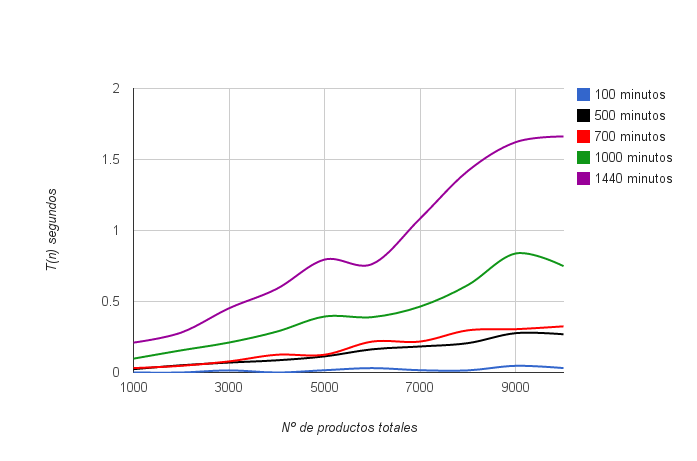
\includegraphics[width=0.8\textwidth]{grafica.png}
	\caption{Representación gráfica de las las pruebas del problema de la planta de producción.}\label{figure}
\end{figure}

\paragraph{}
\begin{center}
	\begin{table}[htbp]
		\centering
		\begin{tabular}{c|c|c|c|c|c}
			N & T(s) 100 M & T(s) 500 M & T(s) 700 M& T(s) 1000 M & T(s) 1440 M \\
			\hline
			1000&	0&			0.023& 	0.031& 0.098 & 	0.211\\
			2000&	0&			0.051& 0.047& 	0.156 & 0.281\\
			3000&   0.015&		0.07& 0.078& 0.211 & 0.452\\
			4000&	0&			0.086& 0.125&	0.288 & 0.589 \\
			5000&	0.016&		0.114& 0.125& 0.394 & 0.795\\
			6000&	0.031&		0.164& 0.218& 0.39 & 0.764\\
			7000&	0.016&		0.183& 0.218& 0.464 & 1.0845\\
			8000&	0.015&		0.207& 0.297& 0.616 & 	1.42\\
			9000&	0.047&		0.277& 0.305 & 0.838 &	1.622\\
			10000&	0.031&		0.269& 0.325 & 0.749 & 	1.662\\

		10000&	1.499&	1.92&	1.419&	1.81&	1.662\\
		\end{tabular}
		\caption{Tiempos medios de las pruebas. }\label{table}
	\end{table}
\end{center}


\begin{thebibliography}{arauak}
	
	\bibitem[cppRef]{key-1} http://es.cppreference.com .
	
	\bibitem[NotasDA]{key-2} https://egela.ehu.es/pluginfile.php/768559/mod\_resource/content/1/NotasDeClase7--12.pdf.
	
	\bibitem[Das]{key-3} Algorithms, S. Dasgupta, C. H. Papadimitriou, and U. V. Vazirani.
	
\end{thebibliography}


\section{Anéxo}
\paragraph{Comentarios:}

\paragraph{}
Las siguientes páginas contienen todo el código utilizado, en lenguaje c++.
\begin{lstlisting}
/* 
* File:   main.cpp
* Author: mikel
*
* Created on 25 de marzo de 2015, 15:47
*/

#include <vector>
#include <cstdlib>
#include <algorithm>
#include <iostream>
#include <fstream>
#include <cmath>
#include <time.h>

using namespace std;

vector<string> pruebas;

typedef struct {
	int tiempo;
	int beneficio;
	int unidadesMax;
	int unidadesSoluccion;
}producto;

typedef struct {
	int beneficioSuma;
	bool pertenece;
	int numProducto;
}valoresF;

int leerFichero(string fname, vector<producto> *pV);
void crearFicheroPrueba(int numProd, int numMinutos , string fname);
void imprimirTablaProduccion(vector<producto> *pV,int pMinutos);
void ejecutarBloquePruebas();
void crearBloquePruebas();
void imprimirSolucion(vector<producto> *pT);
void calcularBeneficioMaximo(string fname);
/*
* 
*/
int main() {
	crearBloquePruebas();
	ejecutarBloquePruebas();
	return 0;
}

void calcularBeneficioMaximo(string fname){
	int Minutos,Ksize = 0, Tj,Bj;
	
	vector<producto> Tabla;
	Minutos = leerFichero(fname,&Tabla);
	
	for(int i = 0; i < Tabla.size(); i++){
		Ksize = Ksize + Tabla[i].unidadesMax;
	}
	
	//Inicializamos la matriz de optimizacion
	valoresF** K;
	
	K = new valoresF* [Minutos+1]; 
	for (int j = 0; j < Minutos+1; j++)    
		K[j] = new valoresF [Ksize+1]; 
	
	//Inicializamos fila y columna 0
	for (int i = 0; i < Ksize+1; i++){
		K[0][i].beneficioSuma = 0;
		K[0][i].pertenece = false;
		K[0][i].numProducto = 0;
	}
	for(int i = 0; i < Minutos+1; i++){
		K[i][0].beneficioSuma = 0;  
		K[i][0].pertenece = false;
		K[i][0].numProducto = 0;
	}
	int i = 0;
	for(int j = 0; j < Tabla.size(); j++){
		Tj = Tabla[j].tiempo;
		Bj = Tabla[j].beneficio;
		for(int k = 0; k < Tabla[j].unidadesMax; k++){
			i++;
			for(int t = 1; t < Minutos+1; t++){
				K[t][i].numProducto = j;
				if( Tj > t){
					K[t][i].beneficioSuma = K[t][i-1].beneficioSuma;
					K[t][i].pertenece = false;
				}else{
					if(K[t][i-1].beneficioSuma < K[t-Tj][i-1].beneficioSuma + Bj){
						K[t][i].beneficioSuma = K[t-Tj][i-1].beneficioSuma + Bj;
						K[t][i].pertenece = true;
					}else{
						K[t][i].beneficioSuma = K[t][i-1].beneficioSuma;
						K[t][i].pertenece = false;
					}
				}
			}
		}
	}
	//Recorremos la matriz incluyendo los elementos que perteneces a la solucion 
	i = Minutos;
	int j = Ksize;
	while((i != 0) and (j != 0)){
		if(K[i][j].pertenece){
			Tabla[K[i][j].numProducto].unidadesSoluccion++;
			i = i - Tabla[K[i][j].numProducto].tiempo;
			j--;
		}else{
			j--;
		}
	}   
	imprimirSolucion(&Tabla); 
};

void imprimirSolucion(vector<producto> *pT){
	for(int i = 0; i < pT->size(); i++){
		cout << pT->at(i).unidadesSoluccion << endl; 
	}
};
/* 
* Input: Nombre de fichero y apuntador al vector de productos 
* Outpu: Rellena array de enteros con los datos del fichero y devuelve en numero de minutos de produccion
*/
int leerFichero(string fname, vector<producto> *pV){
	int i,lines,Minutos;
	ifstream fe(fname.c_str());
	
	fe >> lines;
	if(not(lines > 100 or lines < 1)){
		vector<producto> V(lines);
		for(i = 0; i < lines ; i++){
			fe >> V.at(i).tiempo;
			fe >> V.at(i).beneficio;
			fe >> V.at(i).unidadesMax;
			V.at(i).unidadesSoluccion = 0;
		}
		*pV = V;
		fe >> Minutos;
		fe.close();
		return Minutos;
	}
	fe.close();
	return -1;
};
/* 
* Input: int size, tamano de la lista de elementos, fname nombre para el fichero
* Outpu: Construye un fichero con un entero positivo en la primera linea indicando el numero de lineas
*  que contiene el fichero
*/
void crearFicheroPrueba(int numProd, int numMinutos , string fname){
	int i,tiempo, benficio, unidadesMax;
	ofstream fs(fname.c_str());
	
	fs << numProd << endl;
	for (i = 0; i < numProd ; i++ ){     
		tiempo = 1 + (rand() % 1440);       // Tiempo de produccion posible [ 1 - 1440]
		benficio = 1 + (rand() % 50);     // Beneficio posible [1 - 50]
		//unidadesMax = 1 + (rand() % 10);  // unidadesMaximas posibles [1 - 100]
		unidadesMax = 100;
		fs << tiempo << " " << benficio << " " << unidadesMax << endl;    
	}
	fs << numMinutos << endl;
	pruebas.push_back(fname);
	fs.close();
};
/* 
* Input: vector de productos
* Outpu: imprime por pantalla la tabla de produccion
*/
void imprimirTablaProduccion(vector<producto> *pT,int pMinutos){

	cout <<"Tabla de Produccion"<< endl; 
	cout << endl;
	cout << "N\t" <<"Tiempo\t" << "Benef\t"<< "MaxUnid\t"<< "CantidadOPT\t" << endl; 
	for(int i = 0; i < pT->size(); i++){
		cout << i+1 << "\t"<< pT->at(i).tiempo << "\t" << pT->at(i).beneficio << "\t" << pT->at(i).unidadesMax << "\t"<< pT->at(i).unidadesSoluccion << endl; 
	}
	cout << endl;
	cout << "Tiempo para producir (min):  " << pMinutos << endl;
};

void ejecutarBloquePruebas(){

	clock_t tic,toc;
	for(int i =0; i< pruebas.size(); i++){
		tic = clock();
		calcularBeneficioMaximo(pruebas.at(i));
		toc = clock();
		//cout << pruebas.at(i) << " : " << ((double)(toc - tic) / CLOCKS_PER_SEC)<< " segundos" <<endl;
		cout << ((double)(toc - tic) / CLOCKS_PER_SEC) << endl;;
		if(i == 9 or i == 19 or i == 29){
			cout << endl;
		}
		
	}
};
void crearBloquePruebas(){

	crearFicheroPrueba(10, 100, "10prod500min.txt");
	crearFicheroPrueba(20, 100, "20prod500min.txt");
	crearFicheroPrueba(30, 100, "30prod500min.txt");
	crearFicheroPrueba(40, 100, "40prod500min.txt");
	crearFicheroPrueba(50, 100, "50prod500min.txt");
	crearFicheroPrueba(60, 100, "60prod500min.txt");
	crearFicheroPrueba(70, 100, "70prod500min.txt");
	crearFicheroPrueba(80, 100, "80prod500min.txt");
	crearFicheroPrueba(90, 100, "90prod500min.txt");
	crearFicheroPrueba(100, 100, "100prod500min.txt");

};

\end{lstlisting}


\end{document}
